\documentclass{article}
% pre\'ambulo

\usepackage{lmodern}
\usepackage[T1]{fontenc}
\usepackage[spanish,activeacute]{babel}
\usepackage{mathtools}
\usepackage{graphicx}
\usepackage{listings}
\usepackage{tabu}
\usepackage{hyperref}
\usepackage[utf8]{inputenc}
\usepackage{multicol}
\usepackage{amsmath}
\usepackage{amssymb}
\usepackage{enumerate}
\usepackage{amsthm}
\usepackage{wrapfig}
\usepackage{esvect}
\usepackage{subcaption}
\usepackage{wasysym}
\usepackage[makeroom]{cancel}

\spanishdecimal{.}




% Default fixed font does not support bold face
\DeclareFixedFont{\ttb}{T1}{txtt}{bx}{n}{8} % for bold
\DeclareFixedFont{\ttm}{T1}{txtt}{m}{n}{8}  % for normal

% Custom colors
\usepackage[usenames,dvipsnames]{color}
\definecolor{deepblue}{rgb}{0,0,0.5}
\definecolor{deepred}{rgb}{0.6,0,0}
\definecolor{deepgreen}{rgb}{0,0.5,0}

% Python style for highlighting
\newcommand\pythonstyle{\lstset{
language=Python,
basicstyle=\ttm,
otherkeywords={self},             % Add keywords here
keywordstyle=\ttb\color{deepblue},
emph={MyClass,__init__},          % Custom highlighting
emphstyle=\ttb\color{deepred},    % Custom highlighting style
stringstyle=\color{deepgreen},
frame=tb,                         % Any extra options here
showstringspaces=false            % 
}}


% Python environment
\lstnewenvironment{python}[1][]
{
\pythonstyle
\lstset{#1}
}
{}

% Python for external files
\newcommand\pythonexternal[2][]{{
\pythonstyle
\lstinputlisting[#1]{#2}}}

% Python for inline
\newcommand\pythoninline[1]{{\pythonstyle\lstinline!#1!}}

\usepackage{amsmath} % or simply amstext
\newcommand{\angstrom}{\text{\normalfont\AA}}
\newcommand*{\everymodeprime}{\ensuremath{\prime}}

\title{Tarea 1}
\author{Francisco Felipe Carrasco Varela}

\usepackage{vmargin}

\setpapersize{A4}
\setmargins{1.82cm}       % margen izquierdo
{1.3cm}                        % margen superior
{17.5cm}                      % anchura del texto
{23.42cm}                    % altura del texto
{10pt}                           % altura de los encabezados
{1cm}                           % espacio entre el texto y los encabezados
{0pt}                             % altura del pie de página
{2cm}                           % espacio entre el texto y el pie de página

\usepackage{array,booktabs,tabularx,caption, ragged2e}
\newcolumntype{C}{>{\centering\arraybackslash}X}

\begin{document}
\begin{minipage}{2.3cm}

\includegraphics[width=2cm]{../logo_byn.png}
\vspace{0.5cm}
\end{minipage}
\begin{minipage}{\linewidth}
\textsc{\raggedright \footnotesize
Pontificia Universidad Católica de Chile \\
Facultad de Física -- Instituto de Astrof'isica \\
Astronom'ia -- AST0111 \\
Primer Semestre 2020}
\end{minipage}
\begin{center}
{\LARGE \textbf{Ayudant'ia 1 - Soluci'on}}

\vspace{3mm}

Profesora: Viviana Guzm'an

Ayudantes: Camila Aravena Gonz'alez (\texttt{cfaravena1$@$uc.cl}) -- Francisco Carrasco Varela (\texttt{ffcarrasco$@$uc.cl})

\end{center}
\begin{center}
\noindent\rule{12cm}{0.4pt}
\end{center}


\textbf{Problema 1. Tamaño angular}

\vspace{3mm}

\begin{enumerate} [a)]

\item Si una pelota tiene un di'ametro de $70 \ cm$ y se encuentra a 35 metros de distancia. ?`Qu'e tamaño angular tiene? 

\textit{Soluci'on:}

Para problemas del tama'no angular/di'ametro angular \emph{en astronom'ia}, primero que todo podemos asumir dos cosas:

\begin{enumerate} [i)]
\item Que el objeto que estamos observando es muy peque'nito. Es decir, independiente del tama'no de 'este en la realidad, el objeto tiene un tama'no aparente peque'no dado a que 'este se halla lejos de donde nos encontramos. Por ende trabajaremos con 'angulos peque'nos.
\item Que el objeto que estamos observando es similar a un punto y, por ende, es redondo. De manera que al ser redondo (y parecer una circunferencia) tiene un radio/di'ametro.

\end{enumerate}

Si observamos la Figura \ref{fig1} tenemos el caso en que una persona (ubicada al lado izquierdo de la figura) est'a observando un objeto (ubicado a la derecha de la figura).

Tal cual se dijo, el objeto tiene un di'ametro -el cual llamaremos $D$- y est'a ubicado a una distancia $d$. 

\begin{figure}[!ht]
\begin{center}
\begin{tabular}{ll}
  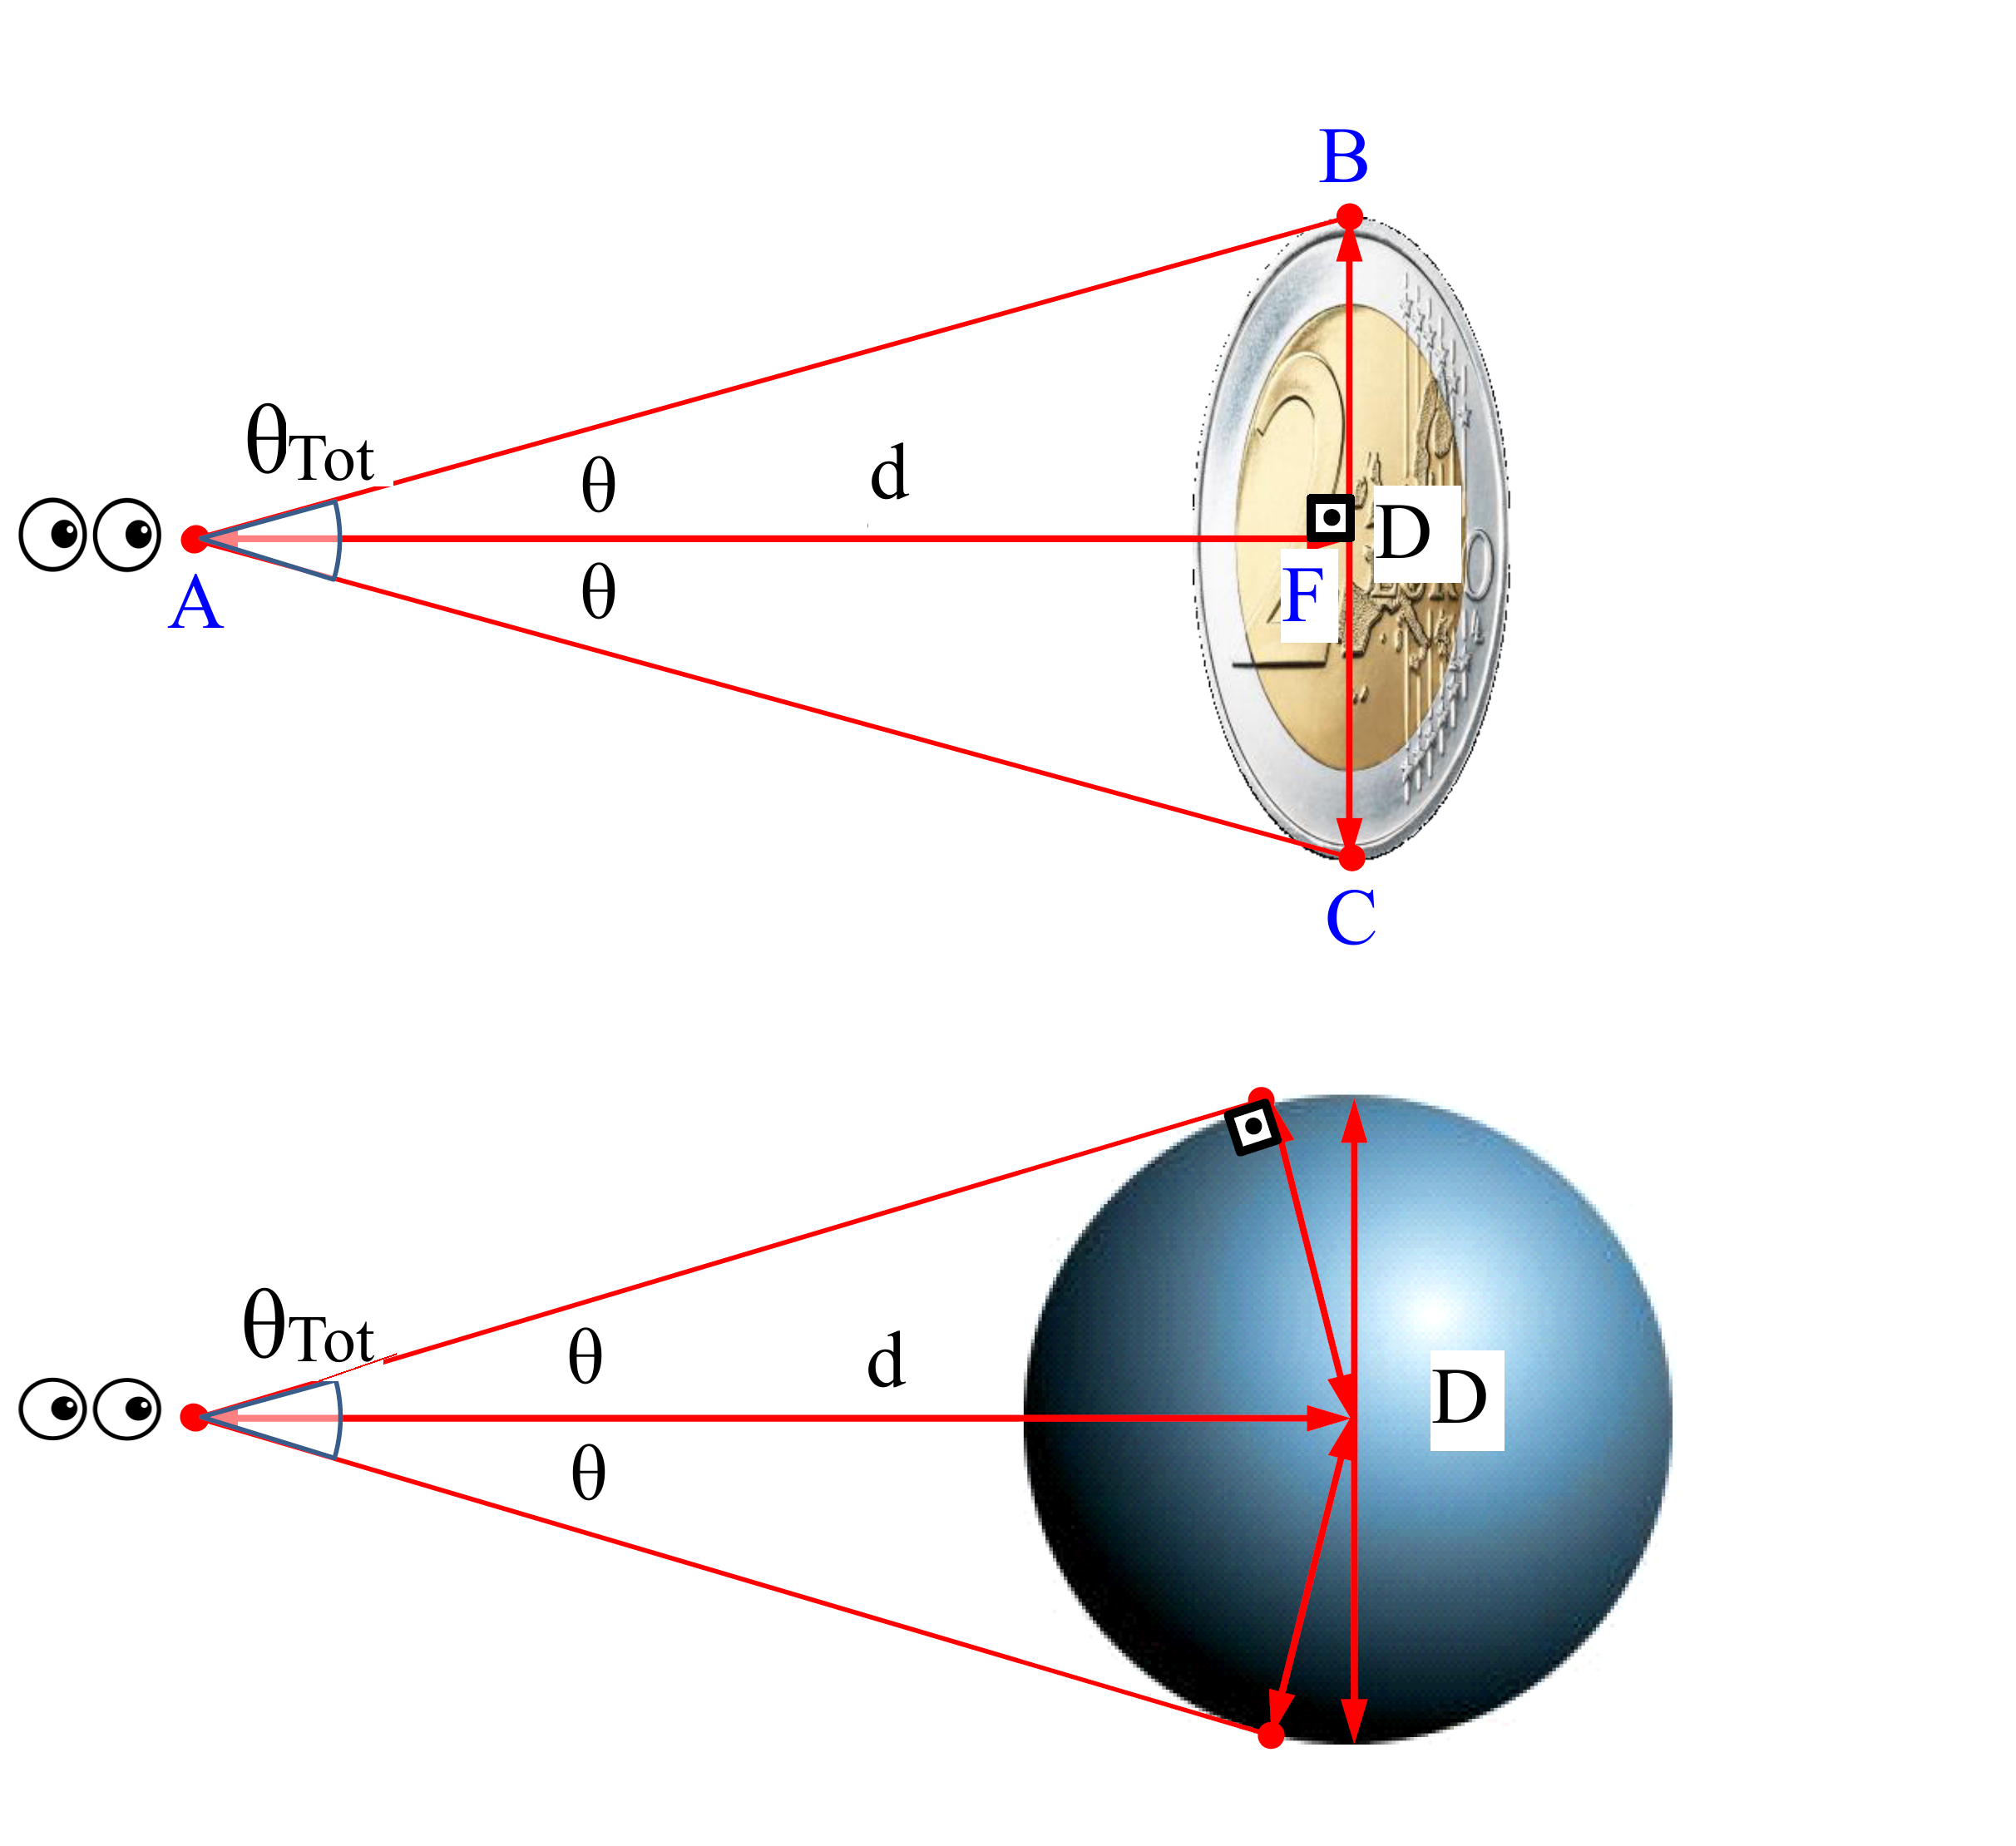
\includegraphics[width=0.4\textwidth]{Diametro_angular.png} 
\end{tabular}
\caption{{\small \textit{Dibujo superior}: Un observador est'a mirando hacia un disco. \textit{Dibujo inferior}: Un observador est'a observando hacia una esfera. El disco/esfera tiene un di'ametro $D$ y est'a a una distancia $d$.
Para 'angulos peque'nos ambos casos son equivalentes. Se recomienda fijarse m'as en el dibujo superior para entender de mejor manera el ejercicio, ya que es m'as simple.}}\label{fig1}
\end{center} 
\end{figure}


Ahora simplemente tratamos de formar un tri'angulo rect'angulo. Para ello formamos un tri'angulo tal cual se muestra en la Figura \ref{fig1}. Aunque, claro est'a, el tri'angulo m'as grande ($\bigtriangleup ABC$) todav'ia no es un tri'angulo rect'angulo. Para formar un tri'angulo rect'angulo, simplemente hacemos una recta entre el observador y el centro del objeto (recta $\overline{AF}$), de manera que ahora s'i se forma un tri'angulo rect'angulo -espec'ificamente dos ($\bigtriangleup ABF$ y $\bigtriangleup AFC$)-, tal cual se muestra en la mism'isima Figura \ref{fig1}. Es claro, entonces, que si el di'ametro del objeto era $D$, entonces su radio es $\frac{D}{2}$ (la mitad del di'ametro).

Hecho esto aplicamos trigonometr'ia pura. Tal cual est'a planteado el ejercicio, lo que deseamos conocer es el tama'no angular del objeto, es decir, el 'angulo total que se forma ($\angle BAC$, o 'angulo de color azul en la Figura \ref{fig1}), el cual llamaremos $\theta_{\text{Tot}}$; ahora bien, al formar los tri'angulos rect'angulos estamos dividiendo el 'angulo $\theta_{\text{Tot}}$ en 2. Este 'angulo que se forma ($\angle BAF$ o $\angle FAC$) en el cualquiera de los dos tri'angulos rect'angulos le llamaremos $\theta$, el cual es igual para ambos tri'angulos rect'angulos. De manera que $\theta_{\text{Tot}} = \theta + \theta = 2 \cdot \theta$. 

?`Qu'e datos conocemos en el problema? El radio del objeto (cateto opuesto del tri'angulo rect'angulo) y la distancia a la que se encuentra (cateto adyacente). Con esto entonces llegamos a la relaci'on trigonom'etrica:

\begin{equation*}
\tan ( \theta ) = \frac{\text{radio}}{\text{distancia}} = \frac{\frac{1}{2}D}{d}
\end{equation*}

O simplemente:

\begin{equation}
\tan ( \theta ) = \frac{1}{2} \frac{D}{d}, \ \ \ \ \ \ |d| \neq 0 
\end{equation}

Para ``despejar'' el 'angulo, $\theta$, aplicamos la funci'on inversa de la tangente a la ecuaci'on, resultando en:

\begin{equation} \label{eq_arctan}
\theta = \arctan \Big( \frac{1}{2} \frac{D}{d} \Big)
\end{equation}

Ahora utilizamos algo que ver'an mucho en la carrera llamado \emph{aproximaciones}. Hay ciertas veces en la vida que uno no tiene una calculadora o computador a mano, o simplemente los c'alculos -incluso usando computadores- son muy tediosos. Es por ello que cuando calculamos ciertas cosas utilizamos ciertos ``life hacks'' para hacernos la vida un poco m'as sencilla y, muchas veces, ahorrarnos la lata de hacer c'alculos muy complicados\footnote{Aunque tampoco abusen de las aproximaciones, traten de hallar un equilibrio. Siempre encontrar'an memes que relacionan las aproximaciones con los ingenieros porque ellos aman las aproximaciones (como usar $\pi = 3$, asies).}.

En este caso en especifico utilizaremos algo conocido como aproximaci'on de 'angulos peque'nos. Si ustedes van a cualquier calculadora que tengan a mano y ponen \texttt{sin(0.1)}, con el 'angulo en radianes, ver'an que la calculadora les arrojar'a un resultado \emph{muy similar} -pero no exactamente igual-  a \texttt{0.1}. ?`Coincidencia? ¡No lo creo! (en C'alculo I o II ver'an porqu'e es as'i). 
Est'a totalmente justificado utilizar esta aproximaci'on en astronom'ia porque principalmente se observan objetos muy pequeños, los cuales no miden m'as de unos pocos grados. 

De manera que la aproximaci'on de 'angulos peque'nos para las funciones trigonom'etricas son:

\begin{itemize}
\item $\sin (x) \approx x$
\item $\cos (x) \approx 1$
\item $\tan (x) = \frac{\sin (x)}{ \cos (x)} \approx \frac{x}{1} = x$
\end{itemize}

Pero recuerden que esto es aplicable \emph{s'i y s'olo si} $x$ es un 'angulo chiquito\footnote{Para la persona que se pregunte a qu'e tan peque'no me refiero con ``chiquito'', estamos hablando alrededor de 'angulos menores a $10^\circ$ o, equivalentemente, $0.174 \ \text{rad}$.}.

Utilizando esta aproximaci'on, la ecuaci'on \eqref{eq_arctan} queda como:

\begin{equation} \label{theta}
\theta \approx \frac{1}{2} \frac{D}{d}
\end{equation}

Finalmente, recordemos que el 'angulo total es $\theta_{\text{Tot}} = 2 \cdot \theta$, de manera que:

\begin{equation}\label{relacion_angulos}
\theta_{\text{Tot}} = 2 \cdot \theta
\end{equation}

Reemplazamos la ecuaci'on \eqref{theta} en la ecuaci'on \eqref{relacion_angulos}, as'i:

\begin{equation*}
\theta_{\text{Tot}} = 2 \cdot \frac{1}{2} \cdot \frac{D}{d}
\end{equation*}

Dando, finalmente:

\begin{equation} \label{angular_size}
\theta_{\text{Tot}} = \frac{D}{d}
\end{equation}

O en español:

\begin{equation} \label{palabras}
\text{Tama{'n}o angular} = \frac{\text{Di'ametro del objeto}}{\text{Distancia al objeto}}
\end{equation}

Para este ejercicio en particular, tenemos que el di'ametro de la pelota es de $70 \ \text{cm}$ y la distancia a ella es de $35 \ \text{m}$. De manera que el ejercicio se resuelve simplemente aplicando la ecuaci'on \eqref{angular_size} hallada:

\begin{equation*}
\theta_{\text{Tot}} = \frac{D}{d} = \frac{70 \ \text{cm}}{35 \ \text{m}} = \frac{0.7 \ \text{m}}{35 \ \text{m}} = \frac{1}{50} = 0.02
\end{equation*}


Si bien la respuesta es ``adimensional'', recordemos que $\theta_{\text{Tot}}$ es un 'angulo. Y, al estar trabajando todo en unidades del Sistema Internacional (S.I.), 'este 'angulo estar'a dado en radianes.
Es decir, y respondiendo a la pregunta de la ayudant'ia, la pelota tendr'a un tama'no angular de aproximadamente $0.02$ radianes cuando se encuentre a $35$ metros de distancia. Algo importante en lo que siempre deben fijarse es en tratar de operar todo en las mismas unidades (mismo sistema de unidades de medida). 

Como tip extra, en astronom'ia trabajamos mucho con 'angulos muy peque'nos. Es por eso que las unidades que se utilizan en este campo para medir 'angulos, m'as all'a de los grados y los radianes, son los arcosegundos; donde arcosegundos se abrevian como ``arcsec'' o como dos comillas. Para que se hagan una idea, un arcosegundo es un grado dividido en 3600. Es decir, $1 \ \text{arcsec} = 1^{\prime \prime} = (\frac{1}{3600})^\circ$. De la misma manera, un radi'an es equivalente a $206265$ arcosegundos, de manera que $1 \ \text{rad} = 206265 \ \text{arcsec}$. Así, la ecuaci'on \eqref{angular_size} puede ser escrita como:

\begin{equation}\label{ang_size_arcsec}
\theta_{\text{Tot}} = 206265 \cdot \frac{D}{d}
\end{equation}

Y la 'unica diferencia entre la ecuaci'on \eqref{angular_size} y la ecuaci'on \eqref{ang_size_arcsec} es que la primera nos entregar'a el tama'no angular en radianes y la segunda nos entregar'a el resultado en arcosegundos, respectivamente.

\item ?`A qu'e distancia debe estar si la quiero ver como un punto, digamos, $10$ veces m'as pequeño? 

\vspace{2mm}

\textit{Soluci'on:}

\vspace{2mm}

Si nos fijamos en la ecuaci'on \eqref{angular_size} o \eqref{palabras}, la cual repito a continuaci'on para su comodidad:

\begin{equation*}
\text{Tama{'n}o angular} = \frac{\text{Di'ametro del objeto}}{\text{Distancia al objeto}}
\end{equation*}

Se ve que el tama'no angular (o di'ametro angular) es directamente proporcional al tama'no del objeto, e inversamente proporcional a la distancia a la cual se halle el objeto.

De manera que si aumentamos 10 veces la distancia, estamos aumentando 10 veces el denominador en el lado derecho de la ecuaci'on y, por tanto, estamos achicando el tama'no angular. De manera que si aumentamos 10 veces la distancia, su tama'no angular ser'a 10 veces menor que la respuesta hallada en la pregunta \texttt{1.a}. Por lo que si queremos ver el objeto 10 veces m'as pequeño, debe estar 10 veces m'as lejos; as'i, la pelota debe estar entonces a $350$ metros de distancia.
\item Pregunta para los curiosos: Por mera casualidad, el Sol y la Luna tienen una relaci'on asociada a su tamaño y distancia. ?`Qu'e nos permite ver esto (que ocurrir'a, por cierto, el 14 de Diciembre de este año)?

\vspace{2mm}

\textit{Soluci'on:}

\vspace{2mm}

Antes de responder la pregunta en s'i, simplemente aclarar algo que les puede servir m'as adelante. En Astronom'ia usualmente la Tierra se simboliza como $\oplus$ y el Sol como $\odot$. Cuando ese s'imbolo va como sub'indice (es decir, como una letra pequeñita abajo a la derecha de una grande), es para indicar la caracter'istica de dicho objeto que va en el sub'indice. Por ejemplo, $R_{\oplus}$ significa el radio de la Tierra. O $M_{\odot}$ significa ``una masa solar''.

Teniendo esto en claro, tenemos que algunos datos que nos sirven para este ejercicio son:

\begin{itemize}

\item $R_\odot= 6.95 \times 10^{8} \ \text{m}$

\item $R_{\leftmoon} = 1.73 \times 10^{3} \ \text{m}$

\item $D_{\oplus \rightarrow \leftmoon} = 3.84 \times 10^{5} \ \text{m}$

\item $D_{\oplus \rightarrow \odot} = 1 \ \text{AU} = 1.49 \times 10^{11} \ \text{m}$ 
\end{itemize}

Donde el tercer dato es la distancia (promedio) entre la Tierra y la Luna, y el cuarto dato es la distancia (promedio) entre la Tierra y el Sol -conocido como Unidad Astron'omica-, respectivamente.
\end{enumerate}

Si vemos cu'antas veces m'as grande es el Sol respecto a la Luna, solamente comparando sus radios, llegamos a lo siguiente:

\begin{equation*}
\frac{R_\odot}{R_{\leftmoon}} = \frac{6.95 \times 10^{8} \ \text{m}}{ 1.73 \times 10^{3} \ \text{m}} = 4.01 \times 10^{5}
\end{equation*}

Pero si ahora vemos cu'antas veces est'a m'as lejos el Sol respecto a la Luna, comparando sus distancias, llegamos a lo siguiente:

\begin{equation*}
\frac{D_{\oplus \rightarrow \odot}}{D_{\oplus \rightarrow \leftmoon}} = \frac{1.49 \times 10^{11} \ \text{m}}{3.84 \times 10^{5} \ \text{m}} = 3.88 \times 10^5
\end{equation*}

?`Qu'e significa esto? Que si bien el Sol es, aproximadamente, unas 400 mil veces m'as grande en tama'no que la Luna; a su vez la Luna est'a unas 400 mil veces m'as cerca a la Tierra en comparaci'on al Sol. ?`Qu'e quiere decir esto? Que colosal diferencia de tama'no se compensa con la cercan'ia del m'as peque'no. Ello quiere decir que si ambos se llegasen a cruzar ser'ian, aproximadamente, del mismo tama'no.

?`Cu'ando se ``cruzan'' estos objetos en cielo? As'i es, señoras y señores, en los eclipses solares. Resaltando esta proporci'on tama'no--lejan'ia en los eclipses solares totales. Gracias a que ambos son, aparentemente, del mismo tama'no es que se ve c'omo la Luna tapa casi perfectamente al Sol. Fue gracias a los eclipses solares totales que se descubrió la parte m'as externa de la atm'osfera del Sol conocida como Corona Solar (y el coronavirus trae su nombre gracias a ella, ya que su forma es muy similar a la Corona Solar\footnote{De manera que si el Sol y la Luna no cumpliesen  esta relaci'on tama'no-lejan'ia quiz'as todav'ia no se hubiese podido descubrir la Corona del Sol cuando al Coronavirus se le puso el nombre y, por ende, tendr'ia otro nombre. Para pensar, señores.}). 

Cabe destacar que esta coincidencia es realmente eso, una coindicencia. Ello quiere decir, por ejemplo, que si alg'un d'ia la humanidad lograse viajar a otro planeta alguna vez y 'este tuviese eclipses solares, ello no garantiza que los eclipses que puedan observar sean totales. Para pensar, ?`no? 
\vspace{3mm}

\textbf{Problema 2. Paralaje}

\begin{enumerate} [a)]

\item ?`Qu'e es el paralaje y para qu'e se utiliza en astronom'ia? Diga, adem'as, sus ventajas y desventajas.

\vspace{2mm}

\textit{Soluci'on:}

\vspace{2mm}

El paralaje es un m'etodo para medir distancia a objetos mediante la trigonometr'ia. En espec'ifico, fij'emonos en la siguiente figura:

\newpage

\begin{figure}[!ht]
\begin{center}
\begin{tabular}{ll}
  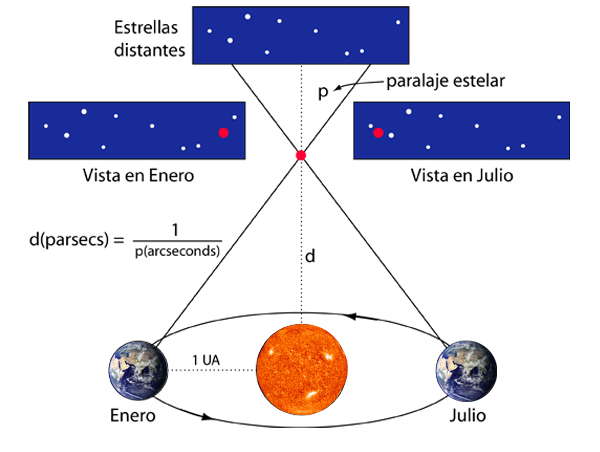
\includegraphics[width=0.4\textwidth]{paralaje.png} 
\end{tabular}
\caption{{\small Idea de paralaje.}}\label{fig2}
\end{center} 
\end{figure}

B'asicamente, el paralaje consiste en lo siguiente:

\begin{enumerate} [i)]
\item Primero tratamos de formar un tri'angulo rect'angulo. En espec'ifico para el caso de medir distancias a estrellas/objetos astron'omicos, para formar el tri'angulo rect'angulo utilizamos la Tierra,  el Sol y el objeto astron'omico que se desea observar.

\item 6 meses despu'es (y asumiendo que la 'orbita de la Tierra alrededor del Sol es exactamente redonda), la Tierra estar'a exactamente ``al otro lado'' de la 'orbita con respecto a donde se encontraba 6 meses atr'as. Se vuelve a formar el mismo tri'angulo rect'angulo.

\item Pero lo que sucede es que el objeto astron'omico aparentemente cambi'o su posici'on en el cielo con respecto a las estrellas del fondo. Esto es lo que llamamos m'aximo cambio de posici'on angular. Pero el paralaje, que llamaremos $p$, es simplemente la mitad de este m'aximo cambio de posici'on angular (tal cual se puede apreciar en la Figura \ref{fig2})

\item Dado esto aplicamos trigonometr'ia: 

\begin{equation}
\tan (p) = \frac{1 \ \text{AU}}{d}
\end{equation}

Ahora, utilizando nuestro nuevo mejor amigo de aproximaci'on para 'angulos peque'nos ($\tan (p) = p$) obtenemos que:

\begin{equation*}
p = \frac{1 \ \text{AU}}{d}
\end{equation*}

Despejando $d$:

\begin{equation*}
d = \frac{1 \ \text{AU}}{p}
\end{equation*}

Y, finalmente, luego de trabajar con las unidades, se llega a la ecuaci'on final:

\begin{equation}\label{paralaje}
d = \frac{1}{p}
\end{equation}

Donde $d$ es la distancia en unidades de p'arsecs; y $p$ es conocido como el 'angulo de paralaje, el cual se encuentra en unidades de arcosegundos. ?`Qu'e es un p'arsec? En estricto rigor se define como la distancia que tendr'ia un objeto cuyo paralaje sea $p = 1^{\prime \prime}$ (un arcosegundo). Un p'arsec (el cual se abrevia como ``pc'') es equivalente a: $1 \ \text{pc} = 3.26 \ \text{ly} = 3.08 \times 10^{16} \ \text{m}$. Es decir, un p'arsec es equivalente a $3.26$ a'nos luz o $30$ mil millones de millones de metros.
\end{enumerate}

\begin{itemize}
\item La ventaja que tiene este m'etodo es que es un m'etodo bastante simple de realizar y, adem'as, es relativamente barato de hacer.

\item La desventaja ser'ia que, para medir distancias, requerimos de una cantidad de tiempo considerable para poder percibir este cambio aparente en el objeto con respecto a las estrellas de fondo. 

Otra desventaja es que, como se puede ver en la ecuaci'on \eqref{paralaje}, la distancia es inversamente proporcional al paralaje. \emph{Esto quiere decir que el paralaje no es 'util para medir distancias a objetos muy lejanos} como, por ejemplo, galaxias. A medida que un objeto se encuentra m'as lejos es cada vez m'as dif'icil medir medir su paralaje. Por ejemplo, misiones actuales/modernas como GAIA -el cual es una especie de observatorio astron'omico espacial- tienen un ``l'imite'' en paralaje hasta 0.04 miliarcosegundos, es decir, su l'imite en paralaje es de aproximadamente $p = 4 \cdot 10^{-5} \ \text{arcsec}$. Por lo que, aplicando la ecuaci'on \eqref{paralaje}, la m'axima distancia que podemos medir con GAIA ser'ian $d = 25000 \ \text{pc} = 25 \ \text{kpc}$. Es decir, si un objeto se encuentra m'as lejos de GAIA que unos $25$ kilop'arsecs, el paralaje ser'a tan peque'no que GAIA no podr'a medirlo y, por tanto, no podr'a estimar la distancia al objeto. 
\end{itemize}

\item ?`Se le ocurre alguna manera ``casera'' de realizar paralaje en su casa?

\vspace{2mm}

\textit{Soluci'on:}

\vspace{2mm}

Un m'etodo muy simple para realizar paralaje en la casa es con el dedo pulgar. Pongan su mano enfrente de ustedes, con los nudillos apuntando hacia adelante y el dedo pulgar extendido hacia arriba. Ahora, mientras observan el dedo pulgar, cierren uno de los dos ojos y mantengan el otro abierto. Sin dejar de mirar el dedo pulgar, cierren el ojo que estaba abierto e inmediatamente abran el ojo que estaba cerrado. Traten de ``intercalar'' el ojo que est'a abierto mientras observan el pulgar y as'i varias veces. Si se dan cuenta su dedo pulgar cambia un poco de posici'on. Esto mismo es lo que aprovecha el paralaje. 

Es m'as, si observan el dedo pulgar cuando acercan su mano mucho a su cara e intercalan el ojo abierto, ver'an que el dedo pulgar cambia mucho su posici'on; pero a medida que vayan alejando su dedo de ustedes, la variaci'on de posici'on del dedo ir'a siendo cada vez m'as peque'na. Una peque'na muestra de que el paralaje, a medida de que las cosas est'an m'as lejos, es m'as dif'icil de percibir y medir.

\item El 'angulo de paralaje para la estrella Sirio es de $p = 1.05 \times 10^{-4} \ ^{\circ}$ (grados). ?`Qu'e tan lejos se encuentra esta estrella de nosotros? (Recuerde siempre tener cuidado con la conversión de unidades)

\vspace{2mm}
\textit{Soluci'on:}
\vspace{2mm}

Recordemos que la ecuaci'on que nos entrega la distancia, la ecuaci'on \eqref{paralaje}, necesita que le entreguemos el 'angulo de paralaje en arcosegundos, pero el enunciado nos entrega el 'angulo de paralaje en grados.

Para saber cu'antos acrosegundos son $1.05 \times 10^{-4} \ \text{grados}$, realizamos una simple regla de 3:

\begin{align*}
& 1^{\prime \prime} \rightarrow \Big( \frac{1}{3600} \Big) ^\circ \\
& x^{\prime \prime} \rightarrow 1.05 \times 10^{-4} \ ^{\circ}
\end{align*}

De manera que $x$ es simplemente:

\begin{equation*}
x^{\prime \prime} = \frac{1^{\prime \prime} \cdot 1.05 \times 10^{-4} \ ^{\circ}}{ \Big( \frac{1}{3600}\Big) ^\circ } = 0.378^{\prime \prime}
\end{equation*}

De manera que el paralaje de Sirio, en arcosegundos, es $p = 0.378^{\prime \prime}$.

Ahora simplemente utilizamos la ecuaci'on \eqref{paralaje}, dando:

\begin{equation*}
d = \frac{1}{p} = \frac{1}{0.378^{\prime \prime}} = 2.64 \ \text{pc}
\end{equation*}

Es decir, Sirio se encuentra a unos $2.64 \ \text{p'arsecs}$ de distancia.


\item Dos personas con mucho tiempo de sobra se ponen de acuerdo para medir la distancia que hay entre la Tierra y Marte aprovechando que estos dos planetas se encontrar'an en oposici'on. Para ello, de aburridos, uno de ellos decide viajar a exactamente el otro lado del mundo (todo esto antes de la cuarentena, por supuesto; ociosos, pero responsables); de manera que la distancia entre los dos es igual al di'ametro de la Tierra\footnote{Radio de la Tierra $\equiv R_{\oplus} = 6.37 \times 10^{6} \ \text{m} \approx 6400 \ \text{km}$ }. El d'ia en que ambos planetas se encuentran en oposici'on, realizan sus mediciones, comparan sus datos de Marte y encuentran que el m'aximo cambio de posici'on angular entre sus mediciones es de $33.6^{\prime \prime}$, ?`cu'al es la distancia, aproximada, entre la Tierra y Marte cuando 'estos est'an en oposici'on? Diga sus respuestas en unidades de metros y AU\footnote{AU $\equiv$ Unidad Astron'omica (de sus siglas en ingl'es) $ = 1.49 \times 10^{11} \ \text{m} \approx 150 \times 10^{6} \ \text{km}$}.

\vspace{2mm}

\textit{Soluci'on:}

\vspace{2mm}

Para empezar, en el enunciado nos dicen que el m'aximo cambio de posici'on angular es $33.6^{\prime \prime}$. Pero, recordemos, el paralaje es la mitad del m'aximo cambio en la posici'on angular del objeto. De manera que, en este caso, el paralaje ser'a:

\begin{equation*}
p = \frac{33.6^{\prime \prime}}{2} = 16.8^{\prime \prime}
\end{equation*}

Basados en la misma idea de paralaje, que es poder medir la distancia bas'andonos en tri'angulos rect'angulos, formamos un tri'angulo rect'angulo entre un observador, el centro de la Tierra y la posici'on aparente de Marte como en la Figura \ref{fig3}.

\begin{figure}[!ht]
\begin{center}
\begin{tabular}{ll}
  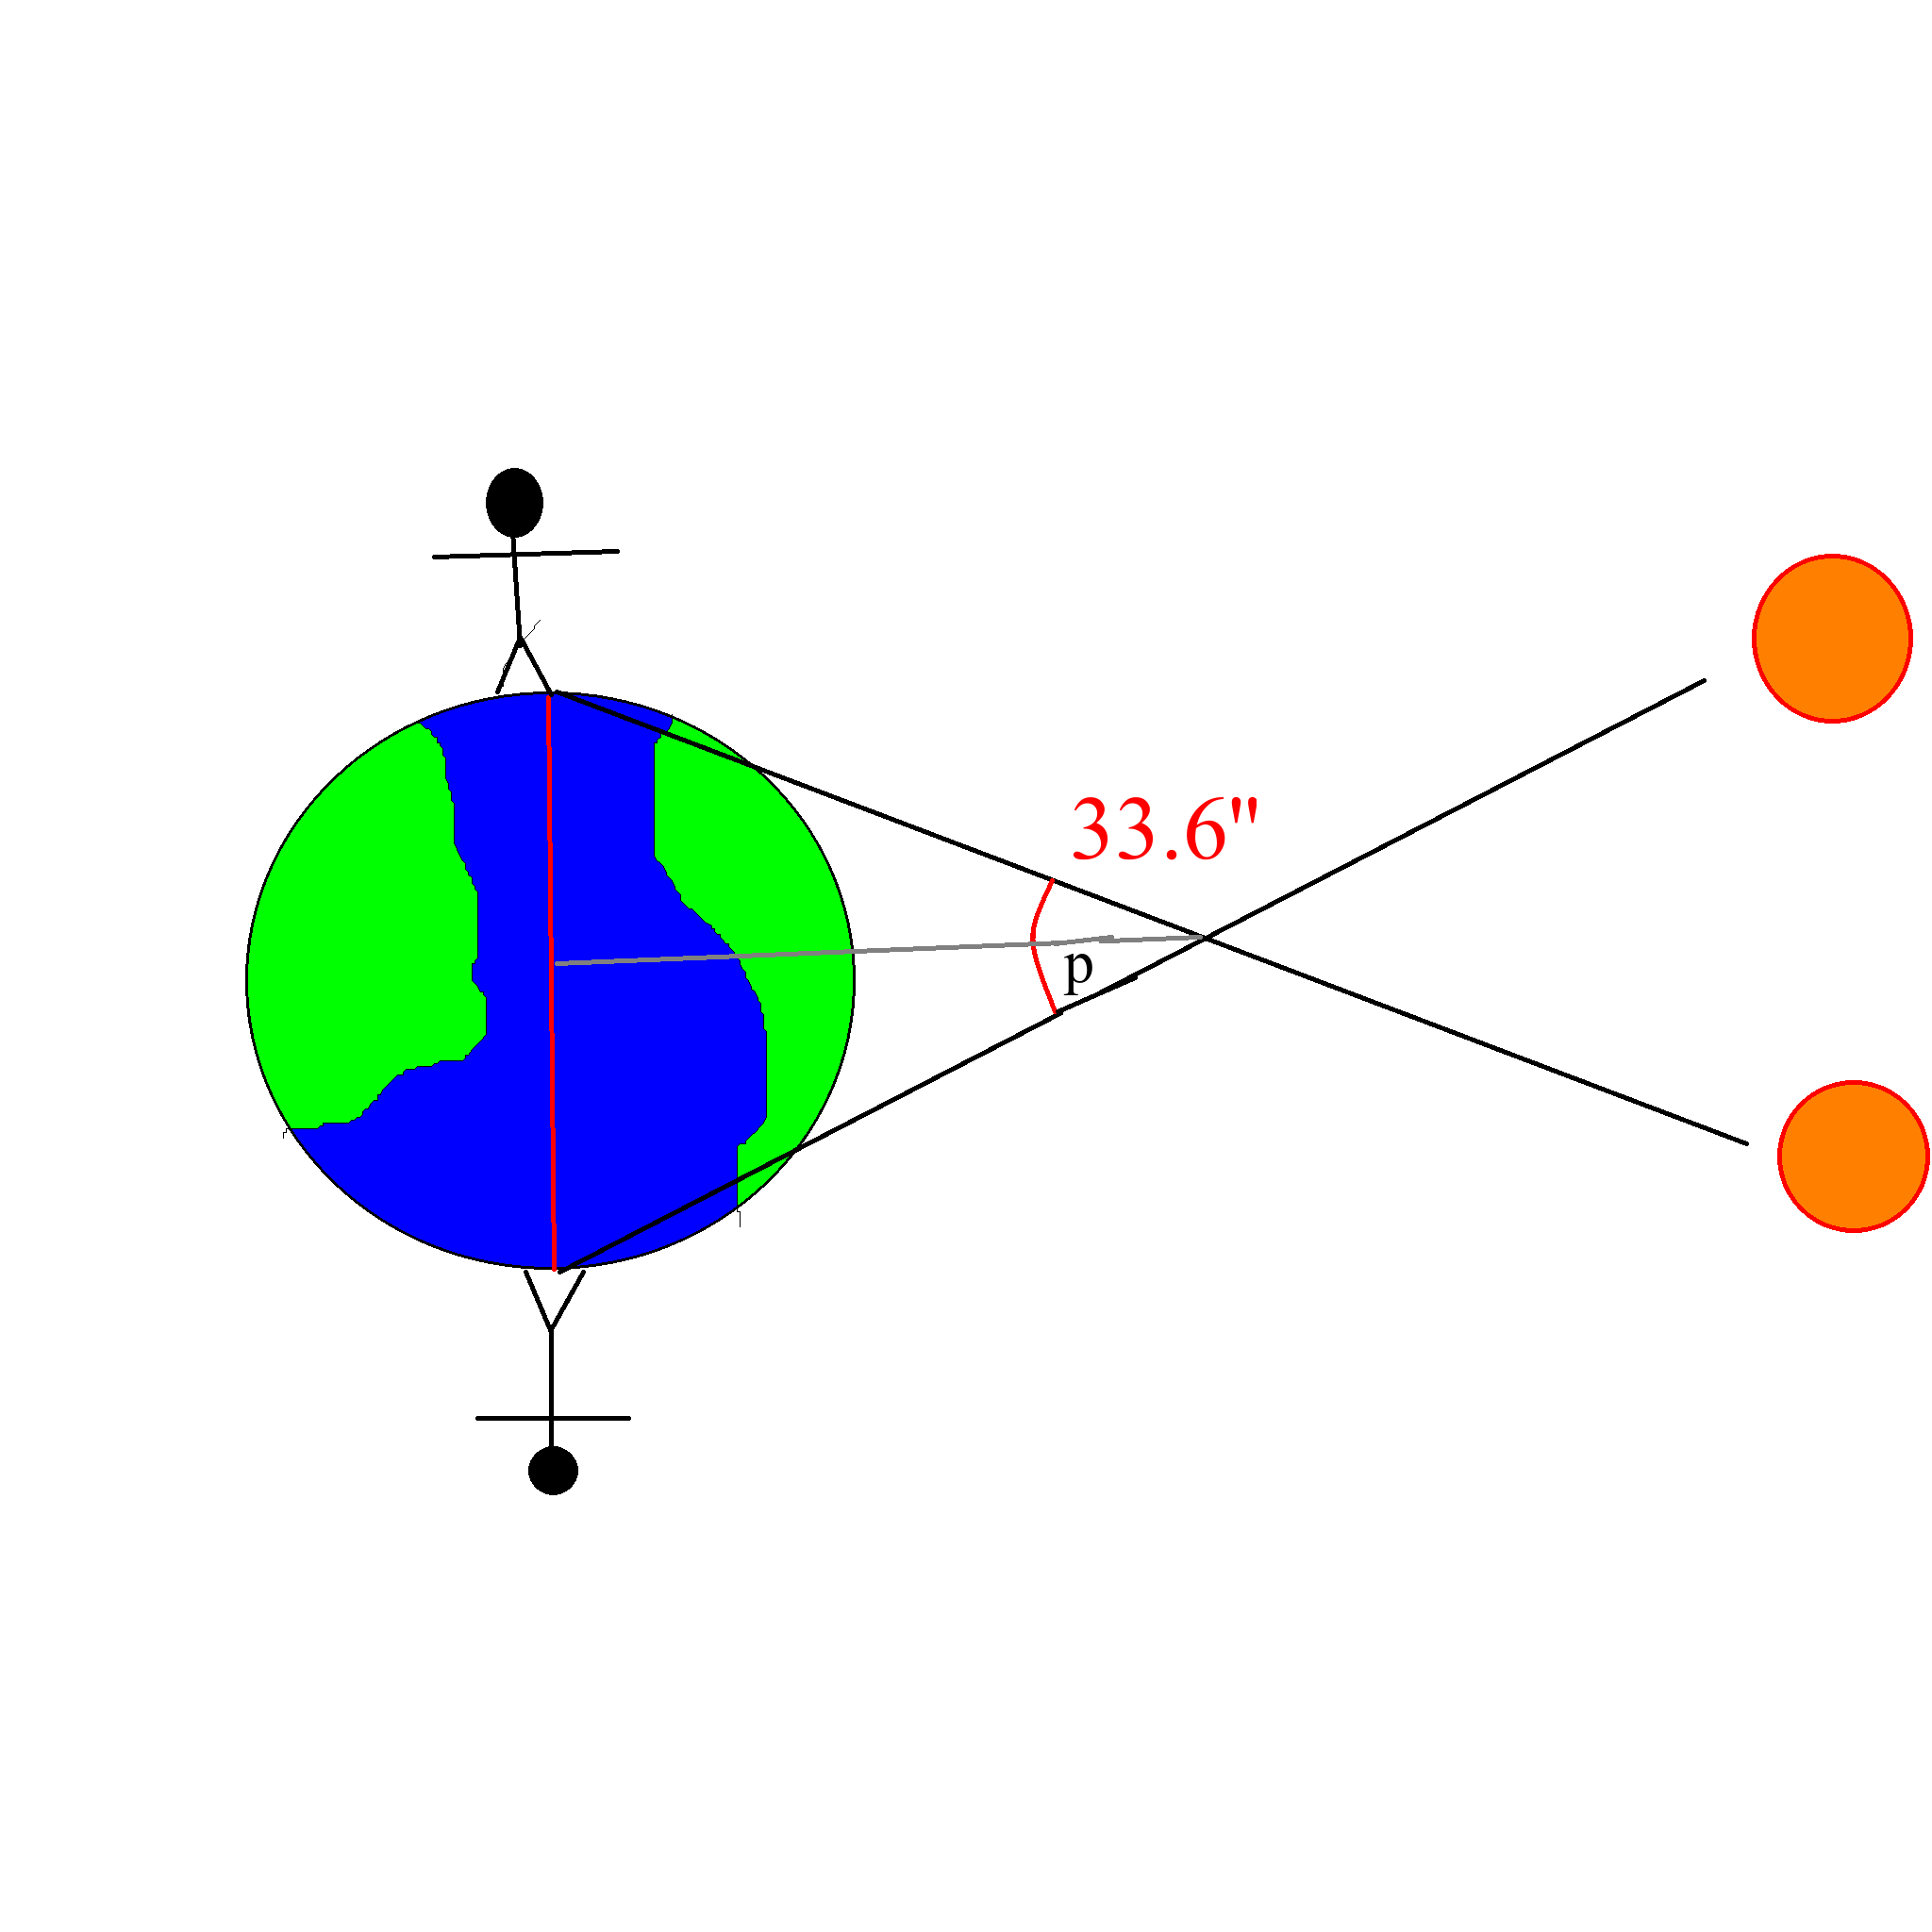
\includegraphics[width=0.5\textwidth]{ejercicio_marte.png} 
\end{tabular}
\caption{{\small Esquema (aproximado) del paralaje para el Ejercicio 2.d.}}\label{fig3}
\end{center} 
\end{figure}

De esta manera volvemos a aplicar trigonometr'ia, obteniendo para el 'angulo de paralaje $p$:

\begin{equation*}
\tan (p) = \frac{R_\oplus}{d}
\end{equation*} 

Utilizando aproximaci'on para 'angulos peque'nos:

\begin{equation*}
p = \frac{R_\oplus}{d}
\end{equation*}

Y despejando la distancia:

\begin{equation} \label{marte_paralaje}
d = \frac{R_\oplus}{p}
\end{equation}

donde $R_\oplus$ es el radio de la Tierra y $d$ es la distancia entre la Tierra y Marte cuando se encuentran en oposici'on (oposici'on es cuando el Sol, la Tierra y Marte forman una l'inea recta; donde la Tierra se encuentra en medio de los dos).

Ahora bien, la ecuaci'on ``original de paralaje'' (ecuaci'on \eqref{paralaje}) no se encuentra en unidades de S.I.. Como en este ejercicio nos piden conocer la distancia en metros, es por ello que para este caso en específico nos conviene trabajar todo en unidades de S.I., ya que as'i la respuesta que buscamos (la distancia) la obtendremos en unidades de longitud del S.I.: metros.

Como queremos todo en unidades de S.I., porque queremos la respuesta en unidades de S.I., pasamos el 'angulo de paralaje a radianes. As'i, se tiene que $16.8^{\prime \prime} \approx 8.18 \times 10^{-5} \ \text{rad}$. Donde tambi'en utilizamos el dato, dado en el enunciado, del radio de la Tierra (en S.I.): $R_\oplus = 6.37 \times 10^{6} \ \text{m}$.

De esta manera, aplicando la ecuaci'on \eqref{marte_paralaje}, obtenemos la distancia Tierra-Marte en oposici'on (que simbolizaremos como $d_{\oplus \rightarrow \mars}$):

\begin{equation}
d_{\oplus \rightarrow \mars} = \frac{R_\oplus}{p} = \frac{6.37 \times 10^{6} \ \text{m}}{8.18 \times 10^{-5}} \approx 7.78 \times 10^{10} \ \text{m} = 0.522 \ \text{AU} 
\end{equation}

Es decir, ambos amigos lograron encontrar que Marte est'a a un poco m'as de media Unidad Astron'omica cuando se encuentra en oposici'on con la Tierra.

\end{enumerate}

\vspace{4mm}

\textbf{Problema 3. Escalas de distancia}

\vspace{2mm}

\begin{enumerate} [a)]
\item Si una nave recorre la distancia que hay entre el Sol y la Tierra en dos años (obviamente, asumiendo que 'esta es pr'acticamente indestructible porque no se derrite, ni deja de funcionar al acercarse al Sol). ?`Cu'anto demorar'a esa misma nave en llegar a Marte, suponiendo que 'esta despega desde la Tierra? Para simplificar el problema, ya que la distancia entre la Tierra y Marte es variable (?`por qu'e?), asuma que los ingenieros hicieron los c'alculos de tal manera que la distancia que recorrer'a la nave es igual a la distancia a cuando la Tierra y Marte est'en en oposici'on; es decir, asuma que la distancia que recorrer'a la nave es igual a la respuesta que hall'o en el ejercicio 2.d).

\vspace{2mm}

Soluci'on:

Recordemos que la definici'on de velocidad es:

\begin{equation}
\text{velocidad} = \frac{\text{distancia}}{\text{tiempo}}
\end{equation}

O:

\begin{equation}\label{velocidad}
v = \frac{d}{t}
\end{equation}

donde $v$ es la velocidad, $d$ es distancia y $t$ es el tiempo.

S'e que estar'a la persona que me dir'a ``...oye, pero esto es la rapidez''. Lo sé. Y est'as bien. Pero para este ejercicio pr'actico, ya que no nos interesa la direcci'on en la que viaja la nave, sino s'olo cu'an r'apido viaja 'esta, velocidad y rapidez son lo mismo para este ejercicio.

Nos dicen que la nave demora alrededor de $2$ a'nos en realizar un tramo desde el Sol hacia la Tierra. Es decir, demora 2 yr (a'no se puede abreviar como ``$\text{yr}$'') en recorrer 1 AU.

La velocidad en principio podr'ia ser $v = 2 \frac{\text{AU}}{\text{yr}}$. Pero en t'erminos pr'acticos ello no nos dice mucho, ¿es ello muy r'apido o muy lento? ?`Cuando ven un auto se mide su velocidad en unidad astron'omica por a'no? No, los medimos en metros por segundo o kil'ometros por hora, por ejemplo. De manera que trataremos de dejar todos los datos que nos dan en unidades del Sistema Internacional. 

As'i, tenemos que 1 a'no son, aproximadamente, $3.15 \times 10^7$ segundos.

Es decir, 

\begin{equation*}
1 \ \text{yr} = 3.15 \times 10^7 \ \text{s}
\end{equation*}

Y 2 a'nos ser'an entonces:

\begin{equation*}
2 \ \text{yr} = 6.3 \times 10^7 \ \text{s}
\end{equation*}

De manera que la velocidad (o rapidez) a la que viaja la nave desde el Sol hacia la Tierra ser'a:

\begin{equation*}
v_{\odot \rightarrow \oplus} = \frac{1 \ \text{AU}}{2 \ \text{yr}} = \frac{1.49 \times 10^{11} \ \text{m}}{6.3 \times 10^{7} \ \text{s}} = 2365 \frac{\text{m}}{\text{s}} = 2.36 \ \frac{\text{km}}{\text{s}}
\end{equation*}

De manera que la nave viaja a $2365 \frac{\text{m}}{\text{s}}$ (o equivalentemente, $8514 \ \frac{\text{km}}{\text{hr}}$).

En el ejercicio anterior, encontramos que la distancia entre la Tierra y Marte (donde simboliz'abamos Marte como $\mars$) era de aproximadamente $d_{\odot \rightarrow \mars} = 7.78 \times 10^{10} \ \text{m}$. De manera que, asumiendo que los ingenieros realizaron los c'alculos correctos de manera que la trayectoria sea la misma del ejercicio anterior y que la nave viaja a velocidad constante (no acelera, ni desacelera), tenemos que el tiempo en que demorar'a en llegar a Marte ser'a:

\begin{equation*}
t = \frac{d}{v} = \frac{7.78 \times 10^{10} \ \text{m}}{2365 \ \text{m} \cdot \text{s}^{-1}} = 3.28 \times 10^7 \ \text{s}
\end{equation*} 

Realizando la conversi'on de segundos a a'nos, obtenemos, finalmente:

\begin{equation*}
t = 3.28 \times 10^7 \ \text{s} \times \Big[ \frac{1 \ \text{yr}}{3.15 \times 10^7 \text{s}} \Big] = 1.04 \ \text{yr}
\end{equation*}

(El paso--ecuaci'on anterior lo puse adrede para mostr'arles c'omo hago yo para pasar de un sistema de unidades a otro. Si alguien se perdi'o en qu'e fue lo que hice, al final de esta ayudant'ia dej'e una especie de ``Ap'endice'' donde explico c'omo lo hago para pasar de un sistema de unidades a otro y el cual les puede servir. No lo hago aqu'i para no perder el hilo del ejercicio.)

De manera que obtenemos que la nave, si mantiene una rapidez constante a lo largo de su viaje, demorar'a un poco m'as de un a'no en llegar hasta Marte.

\item ?`Cu'anto demorar'ian los tramos anteriores (Sol-Tierra y Tierra-Marte) si la nave pudiese viajar a la velocidad de la luz\footnote{Dato ñoño: M'as adelante en la carrera ver'a que es imposible que un objeto con masa viaje a esa velocidad}, es decir, a $3 \times 10^8 \ \text{m}\cdot \text{s}^{-1}$? 
\end{enumerate}

\vspace{2mm}

Soluci'on:

De la ecuaci'on \eqref{velocidad} despejamos el tiempo y obtenemos que:

\begin{equation} \label{tiempo}
t = \frac{d}{v}
\end{equation}

Ahora, si hacemos que la velocidad de la nave sea igual a la velocidad de la luz, es decir, $v = c = 3 \times 10^8 \frac{\text{m}}{\text{s}}$ tendremos que el tiempo de viaje ser'a:

{\begin{small}
$\bullet$
\end{small}}Para el tramo Sol-Tierra:

\begin{equation*}
t_{\odot \rightarrow \oplus} = \frac{1 \ \text{AU}}{c} = \frac{1.49 \times 10^{11} \ \text{m}}{3 \times 10^8 \ \text{m} \cdot \text{s}^{-1}} = 497 \ \text{s} \approx 8.27 \ \text{min}
\end{equation*}

{\begin{small}
$\bullet$
\end{small}}Para el tramo Tierra-Marte:


\begin{equation*}
t_{\oplus \rightarrow \mars} = \frac{7.78 \times 10^{10} \ \text{m}}{3 \times 10^8 \ \text{m} \cdot \text{s}^{-1}} = 259 \ \text{s} \approx 4.32 \ \text{min}
\end{equation*}

Ahora bien, esto en la pr'actica es imposible. Que una nave viaje a la velocidad de la luz no es posible. La respuesta la encontrar'an m'as adelante en un ramo llamado F'isica Moderna.

De igual manera, si nos damos cuenta en lo que se demorar'ia la nave desde el Sol si 'esta pudiese viajar a la velocidad de la luz es alrededor de 8 minutos. Lo que s'i puede viajar a la velocidad de la luz y nos llega desde el Sol son los fotones (luz) que son liberados desde su superficie. Es decir, cuando sea de d'ia, la luz que est'an recibiendo sali'o hace 8 minutos del Sol.




\newpage

\textbf{Ap'endice. Conversi'on de unidades}

\vspace{2mm}

Adem'as de la ``regla de 3'' con la que se pueden obtener los cambios de unidades (como en el ejercicio 2.c), hay una manera que yo utilizo para pasar de un sistema de unidades a otro.

En el Problema 3 les puse una ecuaci'on que era la siguiente:

\begin{equation*}
t = 3.28 \times 10^7 \ \text{s} \times \Big[ \frac{1 \ \text{yr}}{3.15 \times 10^7 \text{s}} \Big] = 1.04 \ \text{yr}
\end{equation*}

Lo cual es lo que hago, en ese ejemplo, para pasar de segundos a a'nos.

Yo hago lo siguiente: En principio tenemos la ecuaci'on original (sin el corchete cuadrado), la cual es el tiempo en segundos:

\begin{equation} \label{ejemplo}
t = 3.28 \times 10^7 \ \text{s}
\end{equation}

Ahora lo que hago es multiplicar por un ``1 m'agico'', pero conveniente. En este caso multiplicamos por $\frac{1 \ \text{yr}}{3.15 \times 10^7 \text{s}}$ en el lado izquierdo de la ecuaci'on superior. ?`Por qu'e esto es multiplicar por 1? Como $1 \ \text{yr} = 3.15 \times 10^{7} \ \text{s}$, podemos darnos cuenta que:

\begin{equation*}
\frac{1 \ \text{yr}}{3.15 \times 10^7 \text{s}} = \frac{3.15 \times 10^{7} \ \text{s}}{3.15 \times 10^7 \text{s}} = 1
\end{equation*}

De manera que al multiplicar la ecuaci'on \eqref{ejemplo} por este 1 conveniente obtenemos la ecuaci'on del problema 3:

\begin{equation*}
t = 3.28 \times 10^7 \ \text{s} \times \Big[ \frac{1 \ \text{yr}}{3.15 \times 10^7 \text{s}} \Big]
\end{equation*}

Si nos damos cuenta, al multiplicar por $\frac{1 \ \text{yr}}{3.15 \times 10^7 \text{s}}$ podemos cancelar t'erminos; en espec'ifico las unidades:

\begin{equation}
t = 3.28 \times 10^7 \ \cancelto{1}{\text{s}} \times \Big[ \frac{1 \ \text{yr}}{3.15 \times 10^7 \cancelto{1}{\text{s}}} \Big]
\end{equation}

Y esto nos queda entonces como:

\begin{equation*}
t = \frac{3.28 \times 10^7}{3.15 \times 10^7} \ \text{yr} = \frac{3.28 \times \cancel{10^7}}{3.15 \times \cancel{10^7}} \ \text{yr} = \frac{3.28}{3.15} \ \text{yr} = 1.04 \ \text{yr}
\end{equation*}

De la misma manera, por ejemplo, si quiero pasar la velocidad de un autom'ovil de metros por segundo a kil'ometros por hora tenemos lo siguiente. 

\begin{equation*}
v = 1 \frac{m}{s} 
\end{equation*}

Multiplicamos por los ``1s convenientes'':

\begin{equation*}
v = 1 \frac{\text{m}}{\text{s}} \cdot \frac{1 \ \text{km}}{1000 \ \text{m}} \cdot \frac{3600 \ \text{s}}{1 \ \text{hora}}   
\end{equation*}

Y ahora simplemente cancelamos y multiplicamos:

\begin{equation*}
v = 1 \ \frac{\cancel{\text{m}}}{\cancel{\text{{s}}}} \cdot \frac{1 \ \text{km}}{1000 \ \cancel{\text{m}}} \cdot \frac{3600 \ \cancel{\text{s}}}{1 \ \text{hr}} = 3.6 \frac{\text{km}}{\text{hr}}   
\end{equation*}

De manera que para pasar de metros por segundo a kil'ometros por hora debo multiplicar por $3.6$.

Entonces, ?`a qu'e me refiero con un ``1 conveniente''? La idea aqu'i es multiplicar por 1s de tal manera que las unidades que se encontraban originalmente en la ecuaci'on se me cancelen con las unidades del 1 conveniente que acabo de agregar, tal cual se vio en el ejemplo anterior.

\vspace{4mm}

\begin{small}
$\bullet$
\end{small}Como un peque'no ejercicio extra, calculemos la masa del Sol en h'amsters. S'i, en h'amsters. 

La masa del Sol es de unos $M_\odot \approx 2 \times 10^{30} \ \text{kg}$. Asumamos, adem'as, que cada h'amster pesa, en promedio, unos $\sim 30 \ \text{gr}$. Para ello tenemos que multiplicar por dos ``1s convenientes''. El primero ser'a $(1 \ \text{h'amster}/30 \ \text{gr})$ y el segundo ser'a $(1000 \ \text{gr}\ / 1 \text{kg})$. 

Tenemos que la masa del Sol es: 

\begin{equation*}
M_\odot = 2 \times 10^{30} \ \text{kg}
\end{equation*}

Ahora multiplicamos por nuestros ''1s convenientes'', de manera que, como mostramos anteriormente, las unidades se cancelen:

\begin{equation*}
M_\odot = 2 \times 10^{30} \ \text{kg} \cdot \frac{1000 \ \text{gr}}{1 \ \text{kg}} \cdot \frac{1 \ \text{h'amster}}{30 \ \text{gr}}
\end{equation*}

Simplificamos todas las unidades que podamos y multiplicamos:

\begin{equation*}
M_\odot = 2 \times 10^{30} \ \cancel{\text{kg}} \cdot \frac{1000 \ \cancel{\text{gr}}}{1 \ \cancel{\text{kg}}} \cdot \frac{1 \ \text{h'amster}}{30 \ \cancelto{\text{bye}}{\text{gr}}} = 2 \times 10^{30} \times \frac{10^3}{3 \times 10} \text{h'amster}
\end{equation*}

Resultando en:

\begin{equation*}
M_\odot = 6.66 \times 10^{31} \ \text{h'amster} 
\end{equation*}

De manera que, realizando conversi'on de unidades, podemos decir que el Sol tiene una masa equivalente entre $10^{31}$ a $10^{32}$ h'amsters. Esos son muchos h'amsters.
\end{document}